\section{Conclusão}
Acreditamos que objetivo principal deste trabalho, implementar um compilador
que pudesse gerar uma representação gráfica da lógica do programa-fonte,
foi cumprido. Temos uma implementação funcional de um compilador que gera
como objetos um programa C e uma representação de grafo em DOT que pode ser
convertido para uma imagem.

Exemplos dos resultados obtidos com o gerador de código C estão demonstrados
na Seção \ref{sec:gen_c} nas Listagens \ref{lst:fib_c} e \ref{lst:fat_c}.
Utilizamos o termo ``exemplos de resultados'' pois não é possível
determinar todos os programas que serão escritos e compilados com nosso
utilitário.

Os resultados obtidos com o gerador DOT não foram, exatamente, aqueles
esperados (verificar discussão na Seção \ref{sec:limitations}). A Listagem
\ref{lst:fib_dot} demonstra o resultado atual da compilação do programa
listado na Listagem \ref{lst:fib} (Fibonacci). A Figura \ref{fig:fibonacci}
demonstra a imagem gerada pela compilação do arquivo DOT.

\lstinputlisting[label=lst:fib_dot, caption=Grafo DOT Fibonacci]{src_files/fibonacci.gv}

\begin{figure}[h!]
	\begin{center}
		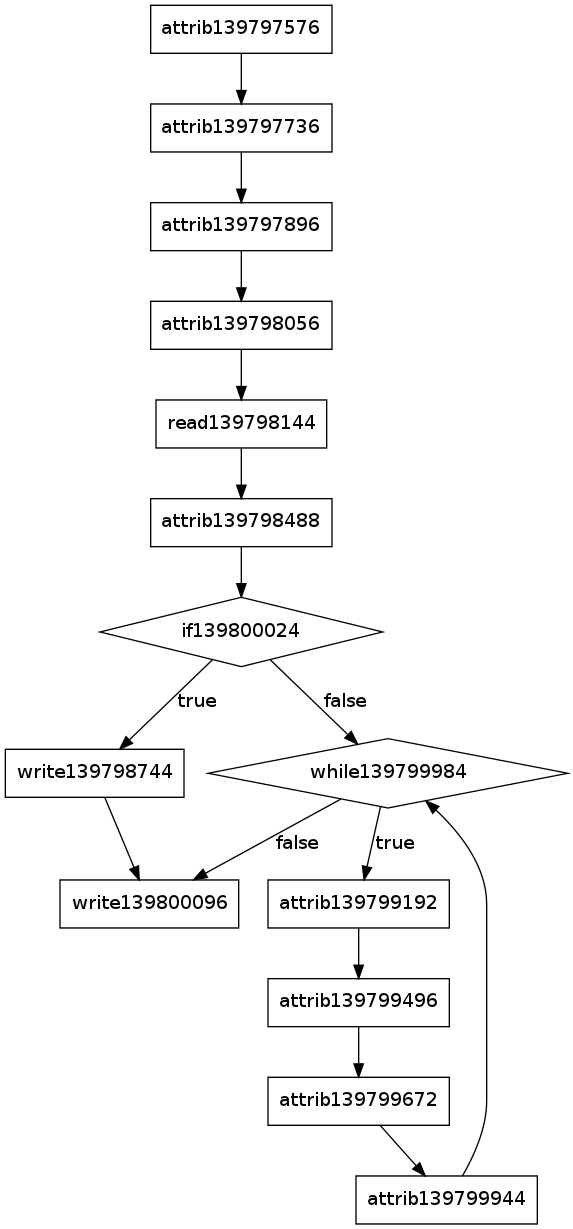
\includegraphics[scale=0.5]{fibonacci}
	\end{center}
	\caption{Representação Gráfica Atual do Programa Fibonacci}
	\label{fig:fibonacci}
\end{figure}

Ainda que não tenhamos obtido, exatamente, o resultado esperado com a
representação gráfica, acreditamos que a ferramenta concebida neste projeto
ainda pode auxiliar programadores novatos em processo de aprendizagem, pois
ainda que de forma limitada, é possível observar o fluxo lógico do programa na
representação gráfica obtida.

O projeto possui outras limitações e possíveis melhorias para suprir essas
deficiências são discutidas na Seção \ref{sec:limitations}. Sugestões para um
próximo projeto de pesquisa são expostos na Seção \ref{sec:suggestions}.


\subsection{Limitações e Melhorias}
\label{sec:limitations}

A limitação principal da gramática, percebida por programadores mais
experientes, é a característica da linguagem operar apenas sobre o conjunto
dos números inteiros. Não há operações de ponto flutuante nem vetores.
Caracteres e cadeias de caracteres (\emph{strings}) também não são
suportados. Acreditamos que programadores novatos, exatamente por serem
novatos, não sejam afetados por essa percepção. Esta limitação de tipos
de dados afetam apenas a geração dos programas-objetos C, pois não criam
novas instruções, apenas novas expressões. Além disso, é possível operar
sobre os novos tipos apenas com as instruções de atribuição, leitura,
escrita, repetição e condicional já implementadas.

A inexistência de definições de procedimentos e ativação de funções é
uma limitação mais severa, pois para que sejam implementadas é necessária
uma alteração profunda da gramática e, por consequência, em todos os
módulos do compilador.

Conforme exibido na Figura \ref{fig:fibonacci}, percebemos que apenas
as instruções são apresentadas na imagem que representa a lógica do
programa-fonte. Os rótulos dos nós apresentam apenas o nome do nó, que
consiste na concatenação nome do seu tipo com o endereço de memória em
que ele estava alocado no momento da compilação. A melhoria consiste em
executar uma passada adicional na árvore sintática para gerar os rótulos
corretamente.

Um exemplo do resultado esperado é apresentado na Listagem
\ref{lst:fib_better}. A respectiva imagem é apresentada na Figura
\ref{fig:fib_better}

\lstinputlisting[label=lst:fib_better,caption=Melhoria Grafo DOT do Programa Fibonacci]{src_files/fibonacci_better.gv}

\begin{figure}[htb]
	\begin{center}
		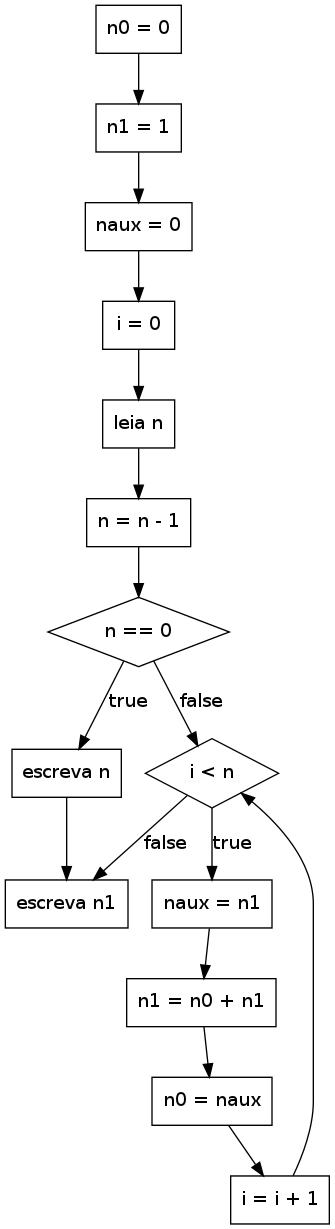
\includegraphics[scale=0.5]{fibonacci_better}
	\end{center}
	\caption{Melhoria da Representação Gráfica do Programa Fibonacci}
	\label{fig:fib_better}
\end{figure}


\subsection{Sugestões para Projetos Futuros}
\label{sec:suggestions}

Com o propósito de nortear a continuidade deste projeto segue uma lista de
sugestões para possíveis melhorias:
\begin{itemize}
	\item Implementar operações para números de ponto flutuante e caracteres;
	\item Implementar estruturas de vetores e matrizes;
	\item Implementar ativação de funções;
	\item Corrigir os rótulos dos nós;
	\item Melhorar a representação gráfica, tornando-a mais parecida com um
	      fluxograma, inclusive incluindo outros formatos para os nós.
\end{itemize}
